\chapter{Modèles de Rea}
	\section{Première modélisation de la performance visuelle relative}
	\par Les sections suivantes décrivent brièvement le contexte et les premiers travaux de Rea qui l'ont mené à proposer sa propre modélisation de la performance visuelle \citep{rea_toward_1986, rea_toward_1987}, définie comme étant la vitesse et la précision atteintes pendant la réalisation d'une tâche visuelle.
	
	\subsection{Modèle précurseur}	
	\par Le premier modèle de Rea est directement inspiré de l'effet de compression proposé par \cite{naka_attempt_1966} qui modélise qu'à partir d'un certain niveau d'intensité, lorsque l'intensité du stimulus augmente, la réponse sensorielle associée augmente de moins en moins jusqu'à atteindre une forme de plateau (voir Fig. \ref{fig:compression_effect}). Les différentes courbes représentent les longueurs d'onde des lumières de couleur utilisées. Cet effet est modélisé de la manière suivante: $\frac{R}{R_{max}} = \frac{I^n}{I^n + k^n}$.
	
	\par Dans cette équation, le rapport de la réponse sensorielle ($R$) sur la réponse sensorielle maximale ($R_{max}$) est égal au rapport de l'intensité $I$ montée à une puissance $n$ déterminée sur la somme de cette même intensité $I$ montée à la puissance $n$ et d'une intensité $k$, également montée à la puissance $n$. La réponse à l'intensité $k$ est égale à la moitié de la réponse sensorielle maximale: $R(k) = \frac{R_{max}}{2}$.
	
	\par On peut faire l'analogie suivante pour donner un bon exemple de l'effet de compression: si dans une pièce on allume une deuxième ampoule d'égale intensité, la sensation de luminosité va grandement augmenter. Au contraire, si on rajoute une ampoule dans une pièce dans laquelle déjà mille ampoules sont allumées, la différence de luminosité perçue sera minime.	
	
	\begin{figure}
		\centering
		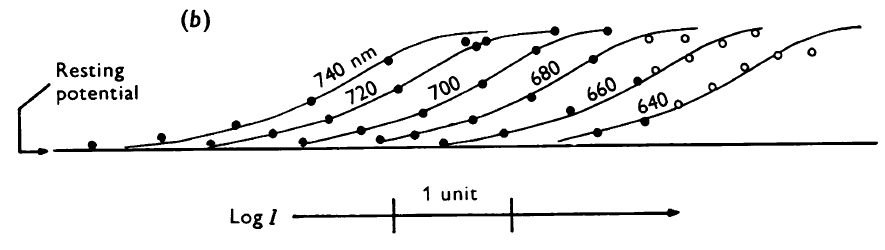
\includegraphics[scale=.6]{Figures/CompressionEffect}
		\caption{Illustration de l'effet de compression.}{Image tirée de \citep{naka_attempt_1966}}
		\label{fig:compression_effect}
	\end{figure} 
	
	\subsection{Application à la performance visuelle}
	\par Rea s'est imposé deux règles pour la conception de son modèle: la performance visuelle doit être issue d'une performance à la réalisation d'une tâche, et le modèle doit être cohérent avec la littérature, notamment avec l'effet de compression que l'on vient de décrire.
	
	\par Le stimulus est décrit (Eq. \ref{eq:rea_contraste}) comme la différence entre le seuil de contraste $C_t$, calculé avec la formule de Blackwell (Eq. \ref{eq:rea_contraste_blackwell}), qui représente le contraste minimal à partir duquel la perception devient possible en fonction de la luminosité du fond ($L_B$) et le contraste visuel $C_V$ qui correspond au contraste entre la luminosité du fond et la luminosité de la tache visuelle ($L_T$) (Eq. \ref{eq:rea_contraste_blackwell}).
	
	\begin{equation}
		C_t = 0.048\left[\left(\frac{0.308}{L_B}\right)^{0.4} + 1.0\right]^{2.5}
		\label{eq:rea_contraste_blackwell}
	\end{equation}
	
	\begin{equation}
		C_V = \frac{L_B - L_T}{L_B}
		\label{eq:rea_contraste_visuel}
	\end{equation}
	
	\begin{equation}
		\Delta C = C_V - C_t
		\label{eq:rea_contraste}
	\end{equation}
	
	\par Les calculs suivants sont ensuite tirés de régressions polynomiales de degré 2 faites avec leurs données expérimentales:
	
	\begin{equation}
		\begin{cases}
		n =  0.882 + 4.38 \theta_1 - 6.05 \theta_1^2\\
		\theta_1 = \log(\log(L_B))
		\end{cases} 
		\label{eq:rea_n}
	\end{equation}
	
	\begin{equation}
		\begin{cases}
		k =  -2.25 + 1.77 \theta_2 - 0.217 \theta_2^2\\
		\theta_2 = \log(L_B)
		\end{cases} 
		\label{eq:rea_k}
	\end{equation}
	
	\begin{equation}
		VP_{max} = 0.0628 + 0.0120 \theta_2 - 0.00268 \theta_2^2
		\label{eq:rea_vpmax}
	\end{equation}
	
	\par Au final, la performance visuelle s'écrit de la manière suivante (Eq. \ref{eq:rea_perfrmance_visuelle}):
	\begin{equation}
		VP = \frac{(\Delta C)^n}{(\Delta C)^n + (k/L_B)^n}
		\label{eq:rea_perfrmance_visuelle}
	\end{equation}
	
	\par Et $RVP = \frac{VP}{f}$ avec $f$ la valeur de $VP_{max}$ dans les meilleurs conditions (luminance et contraste maximaux). Dans le cas de l'expérimentation de Rea, $f = 0.076$.
	
	\par Les résultats de cette expérimentation permettent à l'auteur de dégager trois tendances:
	\begin{itemize}
		\item A contraste constant, la performance augmente avec la luminance,
		\item La performance augmente plus rapidement avec le contraste lorsque les conditions de luminance sont plus élevées,
		\item La performance varie assez peu entre des conditions moyenne et supérieure de contraste.
	\end{itemize}
	
	\section{Méthode des temps de réaction}
	\par Rea et Ouellette complètent la démarche initiale de Rea en proposant une méthode pour établir la performance visuelle d'un sujet, basée sur la mesure et la prédiction des temps de réaction de ce dernier à l'apparition d'un stimulus visuel calibré \citep{rea_visual_1988, rea_relative_1991}. C'est cette modélisation que l'on va chercher à traduire en réalité virtuelle afin de déterminer si elle est utilisable dans le cadre de notre score de réalisme, pour le critère de contraste et de luminance.
	
	\subsection{Protocole expérimental}
	\par L'objectif était de mesurer le temps de réaction de sujets à l'apparition d'une cible sur un écran. La couleur de la cible était calibrée pour obtenir un contraste choisi par rapport au fond sur lequel elle était affichée.
	
	\par L'expérimentation était découpée en deux parties: une première série de mesures pour des cibles plus foncées que le fond sur lequel elles étaient présentées (méthode décrémentale) puis une autre série de mesures avec des cibles plus claires que le fond de présentation (méthode incrémentale).
	
	\par Les cibles, un carré, étaient présentées à $1.68~m$ de l'œil du sujet sur un écran occupant 12 degrés de champ de vision horizontal et 7 degrés de champ de vision vertical. Toutes les cibles étaient vues avec l'œil gauche, à travers un filtre neutre réglable et avec l'ajout d'un voile lumineux artificiel directement au niveau de l'œil (Fig. \ref{fig:rea_apparatus}).
	
	\begin{figure}
		\centering
		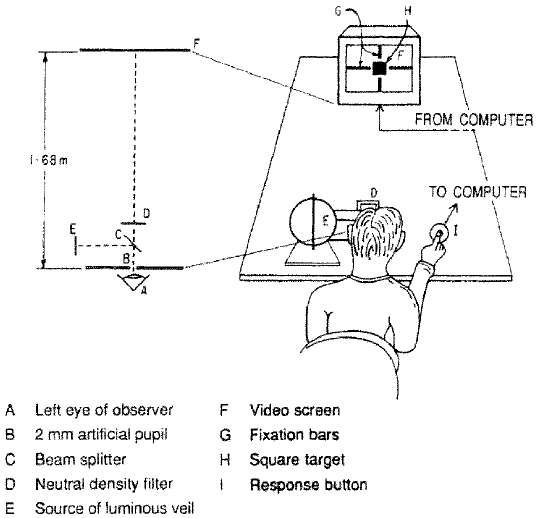
\includegraphics[scale=.75]{Figures/ReactionTimeApparatus}
		\caption{Installation de l'expérimentation de Rea et Ouellette.}{Image tirée de \citep{rea_visual_1988}}
		\label{fig:rea_apparatus}
	\end{figure}
	
	\par Le contraste du carré était calculé en utilisant l'équation suivante (Eq. \ref{eq:rea_ouellette_contraste}):
	 \begin{equation}
		C = \frac{\vert (T L_b + L_v) - (T L_t + L_v) \vert}{T L_b + L_v} = \frac{T \vert L_b - L_t \vert}{L_a}
		\label{eq:rea_ouellette_contraste}
	\end{equation}
	
	\par Avec $T$ la valeur de transmittance du filtre (entre 0 et 1), $L_b$ la luminance du fond de l'écran, $L_t$ la luminance du carré à détecter et $L_v$ la luminance de voile ajoutée artificiellement. $L_a$ représente quant à elle la valeur de la luminance d'adaptation, c'est à dire la valeur pour laquelle l'œil et tout le système optique sont réglés (avec par exemple l'adaptation du diamètre pupillaire).
	
	\par Chaque apparition de cible était espacée d'une temporisation de 1.5 secondes puis d'une temporisation aléatoire variant entre 1 et 3 secondes. La taille de la tache visuelle était variable entre $0.20$ et $280 \times 10^{-5}~steradians$\footnote{Unité sans dimension. un angle solide d'un stéradian délimite sur la sphère unité à partir du centre de cette sphère une surface d'aire 1.}.
	
	\par Chaque sujet a enregistré $19200$ mesures de temps de réaction pour la partie décrémentale et $3625$ mesures pour la partie incrémentale.
	
	\subsection{Calcul des temps de réaction théoriques}
	\par Une fois toutes les mesures effectuées, cela a permis de réétablir une équation de performance avec une protocole similaire à la première modélisation et décrit plus haut. Le détail de ces calculs est présenté en annexes et on retiendra ici seulement l'équation suivante (Eq. \ref{eq:rea_ouellette_performance}):
	\begin{equation}
		R = \frac{(\Delta C_d)^{0.97}}{(\Delta C_d)^{0.97} + K^{0.97}}
		\label{eq:rea_ouellette_performance}
	\end{equation}
	
	\par De cette équation qui décrit la performance du sujet à détecter l'apparition de la tache visuelle en fonction des conditions d'illumination et de contraste, on dérive le temps de réaction en prenant simplement l'inverse de la performance (Eq. \ref{eq:rea_ouellette_reaction_time}):
	\begin{equation}
		RT = \frac{1}{R}
		\label{eq:rea_ouellette_reaction_time}
	\end{equation}
	
	\par Cela permet d'avoir un comportement logique dans les résultats avec un temps de réaction qui diminue quand la performance augmente et inversement.
	
	\par De plus, cette performance $R$ liée au temps de réaction, ainsi calculée, peut être reliée au modèle initial de performance visuelle relative. Cela nécessite d'appliquer deux opérations sur l'ensemble des résultats mesurés dans les deux expérimentations pour les mêmes conditions d'illumination, de contraste et de taille de cible: le calcul de $\Delta T_{vis}$: la variation du temps de réaction par rapport au temps obtenu dans les meilleures conditions expérimentales (Eq. \ref{eq:rea_ouellette_delta_t_vis}). Vient ensuite une transformation linéaire (Eq. \ref{eq:rea_ouellette_linear_transformation}):
	\begin{equation}
		\Delta T_{vis} = RT_{ref} - RT
		\label{eq:rea_ouellette_delta_t_vis}
	\end{equation}
	
	\begin{equation}
		RVP = RVP' \left(\frac{Delta T_{vis} - Delta T_{vis,r}}{Delta T_{vis}' - Delta T_{vis,r}}\right)
		\label{eq:rea_ouellette_linear_transformation}
	\end{equation}
	
	\par Avec $RT_{ref}$ le temps de réaction <<~étalon~>> obtenu dans les meilleures conditions expérimentales, $RVP'$ la valeur maximale de performance visuelle pour le jeu commun de conditions expérimentales, $\Delta T_{vis}'$ la meilleure valeur pour le jeu commun et enfin $\Delta T_{vis,r}$ l'estimation de $\Delta T_{vis}$ au seuil de contraste de lisibilité.
	
	\par On sait donc désormais calculer la performance théorique et donc les temps de réaction théoriques à l'apparition d'une tache visuelle en fonction des conditions de luminance, de contraste et de taille de la cible. Il reste donc à mesurer empiriquement nos propres temps de réactions pour les comparer.
